\documentclass[12pt]{scrartcl}
\title{Assignment 5\\ Video Report\\ Paper Prototyping}
\author{\textbf{Flow Overstack Team}\\ Cesana Filippo\\ Folli Gary\\ Hartmann Kathrin\\ Rodolfo Masera Tommaso\\ Stucchi Jacopo\\ Taillefert Stefano}
\date{}
\setlength{\parindent}{0pt}

\usepackage{graphicx}
\usepackage{float}
\usepackage[margin = 3cm]{geometry}


\begin{document}

\maketitle

\tableofcontents

\newpage

\section{Introduction}

	% Describe briefly the app idea and refer to our concept statement
	
	Our app is a social media which allows its user to discover new information about people who left their footprints in history. Every user-page functions as a box where the historical profiles unlocked by the user are displayed. To unlock a historical profile, firstly the user can take a picture of herself or of another person, and then the app will associate this picture with a historically relevant person, such as Socrate or Abraham Lincoln, for example. Alternatively, the user can unlock this profile through her friends. And here the social side of the app comes into play: when the user decides to share her discovery with her friends, the unlocked historical profile is made visible on the public feed - where all the discoveries achieved by the user friends are displayed.\\
	
	With our app - called V.I.P. - our goal is double. Learning in a funny and social way and challenging a popular nowadays conception of VIP, suggested by other apps like Instagram, where the VIP are often defined as very important for superficial reasons - while of course our VIPs have been selected according to their impact on society, politics, science, philosophy, economy, art, etc.\\
	
	Through a one minute video, we tried to transmit an idea of learning which can defeat boredom by means of the social and interactive nature of our app. For this reason, we divided our video in three parts. In the first one, we depicted two young boys in a state of boredom. We enhanced this feeling by portraying them in very heavy and gloom environments, full of cement and dull colours - and with a plain music playing in background. Then we have the moment of the discovery, during which a third person shows the app to the boys. And finally, on a shining meadow, with a music full of energy, we show social and funny interactions between the two initially bored boys and other young people, thus suggesting that our app, by its funny way to share knowledge, can make the difference when we do not want to feel bored. Of course, after the discovery part, we included in our video also a moving frame in which we show the actual app while it is working.\\
	
	While the premise of our video sounded to us fairly convincing, the feedback that we have collected after having shown the video to two class of young girls and boys was much more eloquent. In the next section, we will dive deeply into the collected data to understand if these two gentle and willing classes, or at least a part of them, actually liked our idea and if our video was clear and persuasive enough to make them like it. 
  
\newpage


\section{Video Feedback Analysis}
	
	% Analyse and report on data gathered with the one minute video exercise and their implications
	% on our design
	
	\subsection{Expectations versus Reality}
	
		% Summarise what we expected from the children and describe the results we actually got
		% through examples/quotes/etc.
		
		TODO (Stefano)
	
	\subsection{Statistics Analysis}
	
		% Spreadsheet of feedback should go in this subsection
		
		INSERT FIRST PAGE HERE (Tommaso)
		
		\subsubsection*{General tendencies - what’s come out of this globally?}

			Before trying to put our data in a numerical form, we can already look at it to get a general tendency. When we speak about general tendency here, we are not talking about the variance, but simply referring to main ideas or opinions that come out of the data. We were able to identify three general tendencies:

				\paragraph{Application useless and potentially boring in the middle/long term} 
					That was, unfortunately, one of the main tendencies. A certain part of the opinions has pointed out that our application would be simply useless or boring relatively quickly. The problem was that in all these opinions, almost no real reason was given. One was pointing out that he prefers playing “real games” than educative apps and another more interesting opinion admitted that even though he found the idea was great, he would be bored quite quickly due to the fact that the picture taking process is repetitive.

				\paragraph{Application very interesting and original for the learning process and the discovery of history through it}
					Fortunately, there was another main tendency, even more present than the first one, that finds the application really interesting and the idea original. The kids pointed out that the learning process embedded in the app under the form of an interactive game would not only be interesting in term of knowledge but also nice for comparing the portrait with other people. Globally, the children seem quite interested by the famous people especially for the history behind them; some opinions stated that it would be a funny way to learn history. Two children said that they found the idea great because they would discover new areas of interest. This process of learning and discovery was one of the main objectives of the app and thus, hopefully, the children seem to agree on that. 

				\paragraph{Partial or total misunderstanding of the application concept}
					A third tendency, less present than the other two is a partial or total misunderstanding of the app. In other terms, the children did not understand the idea behind the app. Some of them were honest and wrote it, while others, through their comments, were taking the app for something else (a scanner, a snapchat filter extension with old portraits, …). And in our opinion, this tendency is even more present that we think for the simple reason that a lot of opinions were binaries, that is to say, “yes” or “no”; thus probably, a part of these children did not understand well the concepts and simply gave “no” as an answer. After having discussed between us, it is true that our video was probably kind of unclear for the children that were not in the front of the class and instead of putting a music with texts, a voice would have probably helped them understanding the app better.
					
					
		\subsubsection*{Quantitative analysis - can we make the data more readable?}

			By definition, qualitative answers like our data are more complex to analyze for the simple fact that they are not numbers (scale, ratio, …) and consequently, constructing graphs and other representations becomes harder. Thus, we had to find a way to convert our data in a quantitative way. We decided to get two main ideas out of the data:\\
			
			Do the child like the app? Would they use it?\\

			Both of these opinions are put on a scale from 0 to 2, 0 being absolutely not, 1 being maybe, 2 being for sure. For every opinion out of the 128, we took the freedom to grade it accordingly to this scale. For us only, we added two more columns, a binary one for the writing (if the child writes correctly or not) and one for the class the child was in (first or second class). We wanted to highlight a potential correlation between their ages or their level at school and their opinions on the app. However, we didn't get any really meaningful correlations. 

			\begin{figure}[H]
                        		\centering
               			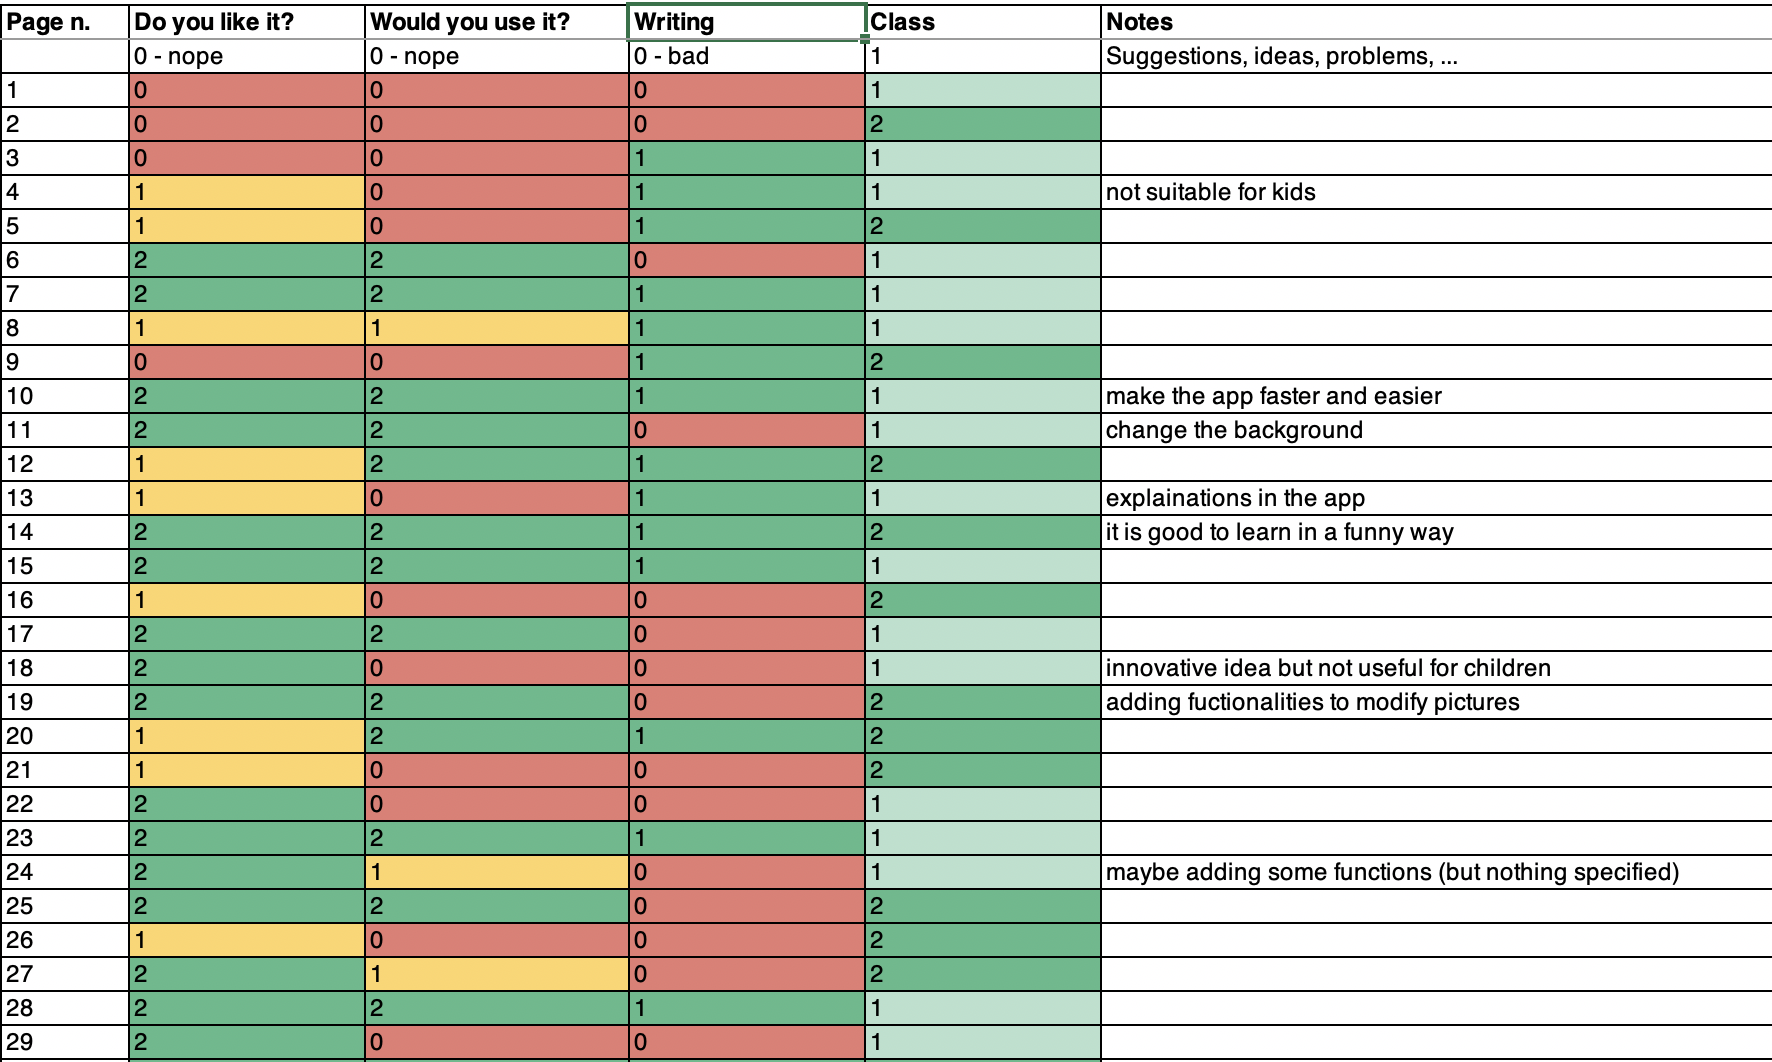
\includegraphics[width=\textwidth]{../images/image_1_data_analysis.png}
               			\caption{Our summarized data}
                        		\label{analysis1}
      			\end{figure}

			Now that we have a quantitative representation, we can build two graphs in order to make a more robust and precise analysis of our data based on the two questions above. We choose to represent the data as histograms and below is the summary of the responses to the first question, “do the children like the app?”.

			\begin{figure}[H]
                        		\centering
               			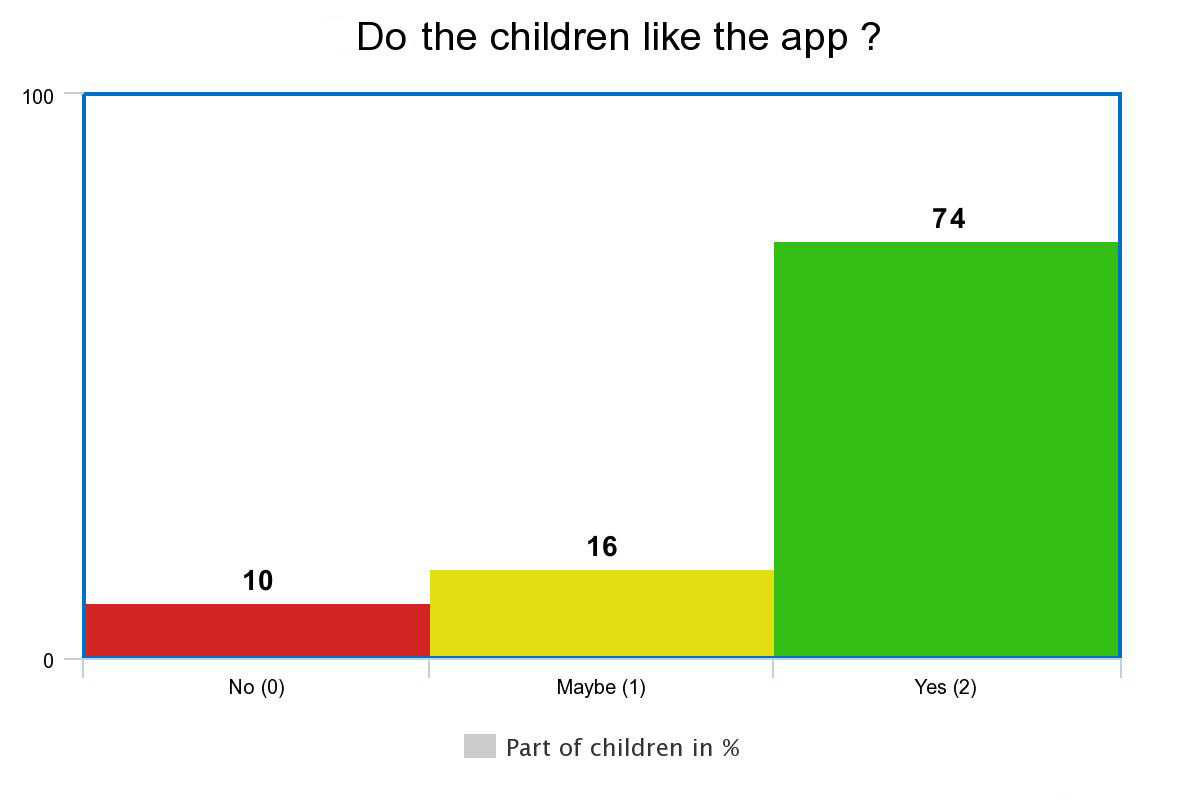
\includegraphics[width=\textwidth]{../images/image_2_data_analysis.jpeg}
               			\caption{The first graph}
                        		\label{analysis2}
      			\end{figure}

			This graph shows a net tendency of children liking the app which really shows that the idea is considered interesting and original. Ignoring those that are undecided, we got a rather good percentage of 74\% against 10\%, which means that the majority like the app and finds it interesting. Now a better question is, “would the children use it?” and here apparently, we get a sharp difference which shows that the children can like an application without planning to use it.\\

			\begin{figure}[H]
                        		\centering
               			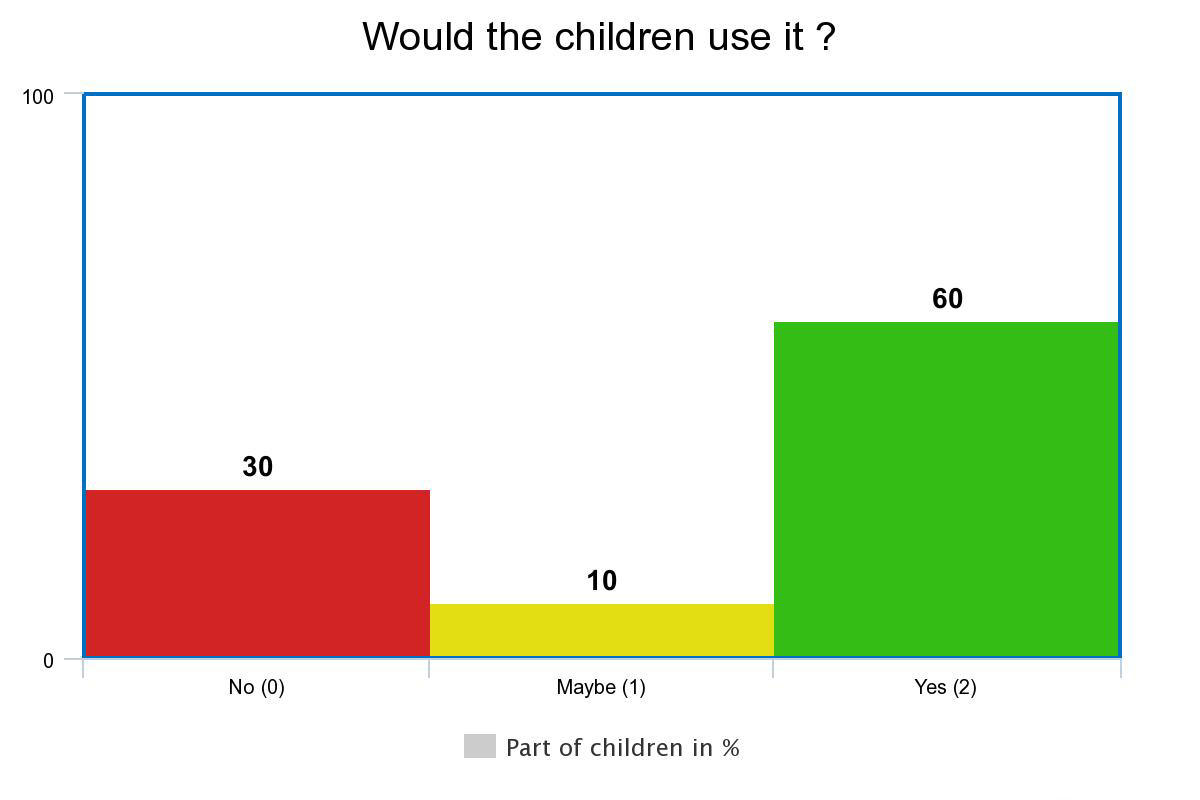
\includegraphics[width=\textwidth]{../images/image_3_data_analysis.jpeg}
               			\caption{The second graph}
                        		\label{analysis3}
      			\end{figure}

			Here the tendency is a bit worse, with a small majority of children that would use it against one third of children that would definitely not use it. For the first question, the ratio liked/non-liked was 7, here the ratio is only 2. Thus, even though the children seem to like the app, they are less excited by the idea to use it. As explained in some opinion, the “educative” side seems to be a barrier; children said that since they are studying enough in school they prefer playing for real on their phone and relaxing rather than continue to learn while playing. We can then clearly see that the response to our app is not unanimous and that even though we try to create a game behind it, the majority of children did not consider it as such.

		
	\subsection{Suggestion-based Improvement}
	
		% Review the kids' feedback and how we plan to modify the project according to it

		Now comes the interesting part, having made the questionnaire in such a way that children were able to develop their answers. Even if the majority did not make any comments on it, we got from some children some really good suggestions and potential improvements for the app. Here are those that were the most noteworthy.\\

		One child was pointing out the fact that characteristics of the person could be added in order to improve the matching process. Although it would somehow break the game aspect, it is true that a variant of our app could have been done to be an educative purpose only application used per classroom in which children were asked to choose proposed characteristics (only positive attributes) of their classmates in order for all children in the class to get associated to a given portraits based on their classmate attributes. The teacher would supervise the process and discuss the results with the children and by doing that children would get in contact with famous people and history though an educative, in-class game.\\
		
		Another child stated that modern VIP should be added in the app as they are more interesting than the past ones. It’s a good idea as modern famous personage would probably add other dimension in the app, like science, biology, physics (with Higgs for example). One of its classmates was also pointing out the possibility to add fictional VIP (from films and series) but that would break the educative aspect of the application (adding Jon Snow from Game of Thrones would be not really useful in term of knowledge and history).\\
		
		Another very good opinion stated that the presence of a search bar would be nice in order to specifically search for a given personage, a bit like a Wikipedia of famous people. That would be an interesting and optional feature for children not interested in the game aspect but more interested by the information and the personages themselves.

	
\section{Paper Prototyping}

	\subsection{Prototype Description}

		% Describe in details the prototype you are creating and how you are going to operate it with 
		% users (peers and children).
		
		TODO (Kathrin \& Tommaso)
		
	\subsection{Key Tasks}
	
		% Show here the list of key tasks (for peers and children) you will use to drive the inspection 
		% process you will run alter on and report in GA6.
	
		TODO (Kathrin \& Tommaso)
			
\section{Conclusion}

	% Describe our expectations for the paper prototype evaluation by the kids/peers
	
	TODO (?)

\end{document}